\chapter{Implementación de un compilador para \textit{tail}}
\label{sect:impl}
Hemos implementado el compilador para el lenguaje \textit{tail} en el lenguaje de programación \textit{OCaml}, utilizando \textit{Opam} y \textit{Dune} para la gestión de dependencias y el control del proceso de compilación respectivamente.\\

\textit{Ocaml} es un lenguaje funcional, basado en \textit{ML} y ampliamente usado en el desarrollo de procesadores de lenguajes gracias a disponer de tipos algebraicos, que facilitan la creación y el trabajo con árboles, contar con optimización para la recursividad de cola, generar código nativo eficiente y soportar diversas librerías útiles para la construcción de analizadores léxicos y sintácticos.\\

Durante la planificación de la implementación se tuvieron en cuenta otras posibles tecnologías. Resumiremos brevemente las razones por las que no fueron elegidas:\\

\begin{itemize}
	\item \textbf{\textit{Haskell}:} Quizá el lenguaje funcional más conocido. Presenta algunas ventajas de las que dispone \textit{Ocaml}, como tipos algebraicos y código nativo eficiente. Sin embargo, el ser un lenguaje funcional puro y la menor disponibilidad de librerías especializadas en lenguajes lo hacen menos conveniente que \textit{Ocaml} para este proyecto concreto.\\
	
	\item \textbf{\textit{Python}:} Es un lenguaje ampliamente usado, con muy buen soporte de librerías de todo tipo y fácil de utilizar. Sería una gran opción de no ser por su bajo rendimiento, que no es admisible en un software del que el usuario espera respuestas rápidas, como lo es un compilador.\\
	
	\item \textbf{\textit{Racket}:} Esta es una opción muy interesante. \textit{Racket} es un dialecto de \textit{Scheme} que proporciona un entorno específicamente pensado para la ``programación orientada a lenguajes'', que propone crear un lenguaje específico para cada problema que quieras resolver. Debido a esto proporciona gran cantidad de herramientas para el procesamiento de lenguajes y la generación de código. El principal problema es que restringe la creación de lenguajes a su plataforma y, como consecuencia, sería necesario que el usuario instalase \textit{Racket} para poder compilar código de \textit{tail}.\\
\end{itemize}

La instalación de \textit{OCaml} dependerá del entorno de trabajo. Las instrucciones se pueden encontrar en \url{https://ocaml.org/docs/install.html}. En entornos Unix es recomendable instalarlo a través de Opam, lo cual puede hacerse mediante la línea de comandos.\\


\textbf{En Ubuntu:}\\

\begin{lstlisting}[style=Consola]
  sudo add-apt-repository ppa:avsm/ppa
  sudo apt update
  sudo apt install opam
  opam init
  eval `opam env`
  opam switch create 4.07.1+flambda
  eval `opam env`
\end{lstlisting}


\textbf{En Debian:}\\

\begin{lstlisting}[style=Consola]
  sudo apt-get install opam
  opam init
  eval `opam env`
  opam switch create 4.07.1+flambda
  eval `opam env`
\end{lstlisting}


\textbf{En Arch Linux y derivados:}\\

\begin{lstlisting}[style=Consola]
  sudo pacman -S opam
  opam init
  eval `opam env`
  opam switch create 4.07.1+flambda
  eval `opam env`
\end{lstlisting}


\textbf{En Fedora, CentOS y RHEL:}\\

\begin{lstlisting}[style=Consola]
  sudo dnf install opam
  opam init
  eval `opam env`
  opam switch create 4.07.1+flambda
  eval `opam env`
\end{lstlisting}


\textbf{En OSX:}\\

\begin{lstlisting}[style=Consola]
  # Instalar Opam mediante Hombrew
  brew install gpatch
  brew install opam
  
  # Instalar Opam mediante MacPort
  port install opam
  
  # Instalar OCaml
  opam init
  eval `opam env`
  opam switch create 4.07.1+flambda
  eval `opam env`
\end{lstlisting}

Igualmente \textit{Dune} pude instalarse mediante \textit{Opam} con el comando \lstinline[style=Consola]{opam install dune}. Con esto ya tenemos todo lo necesario para compilar el proyecto. Posicionándonos en el directorio principal (el que contiene el archivo \textit{tail.opam}) escribiremos las siguientes instrucciones.\\

\begin{lstlisting}[style=Consola]
  # Instalar las bibliotecas necesarias
  opam install . --deps-only
  
  # Compilar el proyecto
  dune build
  
  # Ejecutar tail
  dune exec -- tailc -s <archivo tail a compilar>
\end{lstlisting}

La implementación de \textit{tail} puede dividirse en tres partes: análisis sintáctico, análisis semántico y generación de código. Veamos como se ha desarrollado cada una de ellas.\\


\section{Análisis sintáctico}

La manera estándar de abordar la construcción de un compilador, como bien se explica en \textit{Compilers: Principles, Techniques, and Tools} \cite{dragoonBook}, es separar las fases de análisis léxico, que convierte el código fuente en una serie de tokens, normalmente mediante expresiones regulares y de análisis sintáctico, que toma los tokens proporcionados por el léxico y comprueba que se ajustan a la especificación de una gramática. Para esta tarea se utilizan herramientas especializadas, llamadas lexers y parsers, como las conocidas \textit{lex} y \textit{yacc}.\\

En un principio también seguimos este enfoque, utilizando los equivalentes a \textit{lex} y \textit{yacc} en \textit{OCaml}, \textit{sedlex} y \textit{menhir}. Sin embargo, después de un tiempo qeudó claro que no eran las herramientas adecuadas para un lenguaje como \textit{tail}, que está basado en la identación y utiliza la mínima cantidad de delimitadores posibles (p.e. en las tuplas). Seguía siendo posible usarlas, pero se necesitaba demasiada comunicación desde el parser hacia el lexer, que es algo complicado de conseguir en estos sistemas, haciendo el código difícil de entender y susceptible a errores. Había entonces dos opciones, escribir un parser propio o utilizar una librería de combinadores monádicos.\\

Escribir un parser específico para un lenguaje es algo habitual en lenguajes maduros. Pocos de los lenguajes más conocidos están basados en herramientas generales como \textit{lex} y \textit{yacc}. Eso es debido a la flexibilidad y rendimiento que te proporciona poder adaptar el algoritmo de análisis sintáctico a las necesidades de tu lenguaje. Sin embargo también es la aproximación que más tiempo consume y no es recomendarle usarla cuando la gramática todavía no es estable, ya que un cambio en este tipo de sistemas puede ser muy costoso.\\

Por otro lado los combinadores monádicos son un punto intermedio interesante. Un combinador monádico no es más que un operador que recibe y devuelve una mónada, la cual aísla el estado del sistema permitiendo que el programador se despreocupe de su mantenimiento. Esto en un parser se traduce en que no tienes que lidiar con que posición del archivo estás leyendo o si se ha producido algún error con anterioridad. Una explicación más en profundidad puede encontrarse en \url{https://ocamlverse.github.io/content/monadic-parsers-angstrom.html}. Los combinadores monádicos proporcionan la flexibilidad de un parser específico junto con una comodidad similar a la de generadores de analizadores sintácticos como \textit{yacc}, con la diferencia de que mientras que estos suelen estar limitados a gramáticas $LR(1)$ los combinadores monádicos pueden lidiar con gramáticas $LR(n)$ para un $n$ arbitrario. Esta ventaja también es un inconveniente, ya que la única manera de conseguir esto es mediante backtracking y si no se tiene cuidado la ejecución puede volverse extremadamente lenta.\\

Tras estudiar estas opciones la decisión fue rescribir los analizadores léxico y semántico utilizando la librería de combinadores monádicos \textit{MParser} \cite{mparser}. La implementación se encuentra en el archivo \textit{src/parser/tailparser.ml}. La función que comienza el análisis es \textit{parse}, que recibe un canal de entrada donde se encuentra el código fuente y devuelve un árbol de sintaxis abstracta que está definido por el tipo \textit{expression} en el archivo \textit{src/ast.ml}. Este árbol se utilizará en la fase de análisis semántico.\\

Este árbol se codifica como un tipo algebraico recursivo, que representa la estructura de un programa escrito en \textit{tail} cuando se hace corresponder cada elemento de la gramática con uno de los posibles constructores. Su definición se presenta en el siguiente listado.\\

\begin{lstlisting}[style=ocaml]
type expression = Sequence of info * expression list
| Unit
| Parentheses of info * expression
| Block of info * expression
| BinOp of info * operator * expression * expression
| PrefixOp of info * operator * expression
| PostfixOp of info * operator * expression
| Variable of info * string
| Function of info * string * string list * expression
| Lambda of info * string list * type_expression * expression
| FunctionCall of info * expression * expression option
| Annotation of info * string * type_expression
| VariantDeclaration of info * string * variant_constructor list
| VariantInstance of info * string * string * expression option
| VariantProjection of info * expression * string
| VariantDecomposition of info * string * string * string list
| Assignment of info * string * expression
| If of info * expression * expression
             * expression list * expression option
| Elif of info * expression * expression
| Else of info * expression
| Match of info * expression * (expression * expression) list
| AnyMatch of info
| IntLiteral of info * int
| RealLiteral of info * float
| StringLiteral of info * string
| AtomLiteral of info * string
| BoolLiteral of info * bool
| TupleLiteral of info * expression list
| TupleDecomposition of info * string list
| ListLiteral of info * expression list
| ListDecomposition of info * string * string
| VectorLiteral of info * expression list
| MatrixLiteral of info * expression list list
| DictionaryLiteral of info * (expression * expression) list
\end{lstlisting}

De esta forma una expresión como ``\lstinline[style=tail]{x := 1}'', se correspondería con\\ ``\mbox{\lstinline[style=ocaml]{Assignment(i, "x", IntLiteral(i, 1))}}''. Donde ``i'' contiene cierta información, como la posición del archivo donde se ha leído la expresión, que será útil para proporcionar mensajes de error de calidad.\\

Por último ilustramos con un ejemplo el funcionamiento de \textit{MParser}, definiendo la regla para identificar un entero y construir su representación en el árbol sintáctico.\\

\begin{lstlisting}[style=ocaml]
let decimal = many1_chars digit

let int_literal =
	get_pos >>= fun sp -> decimal
	>>= fun s -> get_pos
	>>= fun ep -> return (IntLiteral (pos_info sp ep, int_of_string s))
\end{lstlisting}

La primera regla que definimos es \textit{decimal}, que hace uso de dos combinadores proporcionados por la librería: \textit{digit} identifica cualquier caracter del ``0'' al ``9'' y lo devuelve como una mónada de tipo \textit{char}, por su parte \textit{many1\_chars} intenta aplicar la regla \textit{digit} varias veces y devuelve el resultado como una mónada de tipo \textit{string}. De esta forma podemos identificar cualquier sucesión de caracteres numéricos.\\

La regla \textit{int\_literal} hace uso del operador $>>=$, que se corresponde con la función \textit{bind} habitual de las mónadas. Este operador presenta la siguiente signatura:

\begin{center}
	\lstinline[style=ocaml]{val (>>=): ('a, 's) t -> ('a -> ('b, 's) t) -> ('b, 's) t}
\end{center}

La notación \lstinline[style=ocaml]{('a, 's) t} hace referencia a una mónada de tipo \lstinline[style=ocaml]{'a} con un estado de tipo \lstinline[style=ocaml]{'s}. Por tanto ese operador acepta como parámetros una mónada de tipo \lstinline[style=ocaml]{'a} y una función que transforma un elemento de tipo \lstinline[style=ocaml]{'a} a una mónada de tipo \lstinline[style=ocaml]{'b}, devolviendo una mónada de tipo \lstinline[style=ocaml]{'b}. La idea intuitiva detrás de esto es que $>>=$ toma una mónada y una función, rescata el elemento guardado en dicha mónada y le aplica la función para, a continuación, guardar el resultado en una nueva mónada y devolverla.\\

Sabiendo esto lo que se hace en el ejemplo es aplicarle a la mónada \textit{get\_pos} (que guarda la posición actual de lectura) una función que le aplica a la mónada \textit{decimal} otra función que le aplica a otra mónada \textit{get\_pos} (para obtener la posición final de lectura) una última función que devuelve una mónada que guarda una representación de un entero en el árbol sintáctico. O más sencillo: se obtiene la posición inicial y se le da como nombre ``sp'', se reconoce una secuencia de números y se le da como nombre ``s'', se obtiene la posición final y se le da como nombre ``ep'' y por último, utilizando estos datos se construye el tipo \textit{IntLiteral}.\\

El resto de reglas del análisis sintáctico siguen los mismos principios, haciendo uso cuando es necesario de otras primitivas y operadores proporcionados por \textit{MParser}.\\


\section{Análisis semántico}

Esta fase consiste en la comprobación de que el código no solamente se adhiere a las normas de la gramática, sino que además tiene sentido. Para ello hay que asegurarse de que, por ejemplo, no se utilicen variables o funciones que no han sido declaradas en el scope actual o uno superior. En \textit{tail} tampoco se permite utilizar una variable que no ha sido inicializada con un valor, esto también hay que vigilarlo. Es también en esta fase donde se implementa el sistema de tipos, comprobando que todas las expresiones están tipadas de forma correcta de acuerdo a las especificaciones de las reglas de tipado.\\

Para llevar a cabo esta serie de checkeos es necesaria una estructura donde ir guardando la información, la cual cumple la misma función que el contexto $\Gamma$ en las reglas de derivación. Esta estructura se llama tabla de símbolos y es un elemento estándar a la hora de implementar algún tipo de analizador de lenguajes \cite{dragoonBook}. La forma más simple de implementar una tabla de símbolos es utilizar una lista en la que se van introduciendo entradas tales como declaraciones de variables o de funciones, junto con una entrada especial $Block$ que delimita cuando comienza un nuevo scope. De esta forma para comprobar que una variable sea válida solo hay que comprobar que se encuentre en la lista y en el momento en que al recorrer el árbol sintáctico se sale del scope actual se borran todas las entradas hasta la última marca $Block$. Sin embargo esta técnica no es adecuada para lenguajes que necesitan de varias pasadas al árbol sintáctico como \textit{tail}. Dado que en \textit{tail} una función puede ser referenciada incluso antes de que se declare, siempre que sea accesible en ese scope, se necesita de una primera pasada para localizar a todas las funciones, pero esto no serviría de nada si después de recorrer el árbol todas las funciones han sido eliminadas de la tabla de símbolos. La solución a esto es utilizar una estructura recursiva en forma de árbol. Una tabla de símbolos tiene a su vez una lista de tablas de símbolos hijas que almacenan los símbolos accesibles en scopes inferiores. De esta forma, para comprobar si una variable es válida, se busca primero en la tabla actual y si no se encuentra se busca en las tablas padre. Esto evita el uso del marcador $Block$ y la necesidad de borrar entradas al salir de un scope. La implementación de la tabla de símbolos se encuentra en el archivo \textit{src/semantic/symbols\_table.ml}.\\

En \textit{tail} las tareas de comprobación se han dividido en cuatro funciones. Primero la función \textit{fill\_predefined}, definida en \textit{src/semantic/scopechecker.ml} rellena la tabla de símbolos con variables y funciones predefinidas del lenguaje. A continuación \textit{fill\_constants}, en el mismo archivo, recorre el árbol buscando variables declaradas como constantes, que en la implementación actual de \textit{tail} son únicamente la declaración de funciones, y las introduce en la tabla de símbolos, haciendo posible que se referencien incluso antes de su declaración siempre que se haga desde el scope adecuado. Ahora se llama a \textit{scope\_check}, también en \textit{src/semantic/scopeckecker.ml}, que se encarga de comprobar que todas las referencias a variables y funciones son válidas. Por último se utiliza \textit{type\_check}, que reside en el archivo \textit{src/semantic/typechecker.ml}, para revelar cualquier inconsistencia en el tipado. La coordinación de estas funciones se encuentra en el archivo \textit{src/semantic/tailsemantic.ml}, concretamente en la función \textit{check\_semantics}, que recibe como parámetro el árbol construido en la fase de análisis sintáctico.\\

El resultado de todas estas operaciones es un nuevo árbol sintáctico en la que esta vez, cada expresión está decorada con su tipo correspondiente y que se utilizará en la fase de generación de código.\\

Al igual que en apartado anterior explicaremos el funcionamiento de esta fase con un ejemplo simple. El siguiente fragmento de código forma parte de la comprobación de scope:

\begin{lstlisting}[style=ocaml]
let rec scope_check (ast:Ast.expression) (st:symbols_table) =
	match e with
	
	...
	
	| Assignment (i, n, e) ->
		let check_e st =
			begin match scope_check e st#next_child with
			| Ok new_st ->  Ok st
			| e -> e
			end
		in
		begin match st#find_variable_in_scope n with
		| Some (VariableEntry (n, t, init)) ->
			st#update_entry (VariableEntry (n, t, init))
			                (VariableEntry (n, t, true));
			check_e st
		| _ ->
			st#add_entry (VariableEntry (n, Unknown, true));
			check_e st
		end
	
	| Variable (i, n) ->
		begin match st#find_variable n with
		| Some v ->
			begin match v with
			| VariableEntry (n, _, false) -> Error (i, Printf.sprintf "The variable %s is not initialized." n)
			| _ -> Ok st
		end
		| None -> Error (i, Printf.sprintf "%s doesn't exist." n)
	end
\end{lstlisting}

Cuando recorriendo el árbol el programa se encuentra con una asignación, lo primero que hace es comprobar si la variable a la que se le va a asignar el valor existe en la tabla de símbolos. Si es así la actualiza para que figure como inicializada (líneas 15 y 16), si no existe la añade directamente. Por último continúa con el análisis de la expresión derecha de la asignación (línea 20), en este caso utilizando la tabla de símbolos hija de la actual, representando la entrada a un scope inferior (línea 8, \lstinline[style=ocaml]{st#next_child}).\\

En caso de encontrarse con una variable, comprueba que esta sea accesible desde el scope actual buscándola en la tabla de símbolos (línea 24). En caso de que no se encuentre devuelve el error correspondiente (línea 30). Si todo va bien comprueba que la variable está inicializada, algo que hemos hecho en la regla de asignación, y termina el análisis con un mensaje de error en caso de que no lo esté, o con la tabla de símbolos actualizada.\\

\section{Generación de código}
La fase de generación de código iba, en un principio, a apoyarse en el proyecto LLVM \cite{llvm}. Este proyecto proporciona una serie de herramientas para facilitar la programación de compiladores, las más destacables son: un lenguaje, a medio camino entre ensamblador y \textit{C}, pensado para ser utilizado como representación intermedia, un compilador que traduce este lenguaje a código máquina y una serie de librerías que facilitan la conversión del lenguaje original a dicha representación intermedia.\\

Las ventajas de utilizar LLVM son numerosas. Por un lado, una vez que has traducido tu lenguaje a la representación intermedia, puedes compilarlo a cualquier arquitectura soportada por el proyecto. Esto quiere decir que puedes disponer de código nativo sin sacrificar en portabilidad ni tener que aprender y generar el código ensamblador específico de varios sistemas. Además LLVM también proporciona herramientas para la optimización de código e incluso para añadir recolección de basura.\\

El funcionamiento básico sería sencillo: el compilador de tail recorrería el árbol sintáctico generando el lenguaje de representación intermedia. Este código intermedio, a su vez, sería traducido a código máquina gracias al compilador de LLVM. Sin embargo, se presentó una dificultad inesperada que no ha podido ser salvada. El código intermedio de LLVM es fuertemente tipado, esto quiere decir que para generarlo es necesario conocer los tipos de las variables y las funciones en tiempo de compilación, lo cual es incompatible con el tipado gradual de \textit{tail}. Además, la única solución que se ofrece para la compilación de lenguajes con tipado dinámico, el ``bitcasting'' (cambiar el tipo de los punteros para que acepten el valor asignado), no solo dificulta la implementación en gran medida, obligando a utilizar punteros en todas las variables, sino que además no funciona como debería, provocando problemas con la reserva de memoria. Este inconveniente se supone que será solucionado en próximas versiones, con la llegada de punteros opacos, pero actualmente LLVM no es una herramienta adecuada para lenguajes que no estén fuertemente tipados.\\

Tras invertir un tiempo considerable aprendiendo LLVM y realizando parte de la implementación y con el tiempo disponible reduciéndose, opinamos que lo más prudente era no realizar la fase de generación de código. Aunque esto suponga no completar totalmente uno de los objetivos, esta no constituye un elemento imprescindible del trabajo, siendo la parte fundamental del TFG el sistema de tipos.\\


\section{Ejemplos de ejecución}
Tras la explicación de la implementación vemos necesario validar su correcto funcionamiento. Para ello ofreceremos varios ejemplos de la ejecución del compilador con diferentes fragmentos de código, tanto correcto como incorrecto, para mostrar el comportamiento del programa.\\

El primer ejemplo consiste en una sencilla implementación de la sucesión de Fibonacci. Este código se puede encontrar en el archivo \textit{tests/test\_files/fibonacci\_1.tail}.\\
\newpage

\begin{lstlisting}[style=tail]
fib : Int -> Int
fib(n) :=
	if n <= 1 then
		1
	else
		fib(n-1) + fib(n-2)

write("fib(3) = {fib(3)}")
\end{lstlisting}

El código es totalmente correcto, por lo que sería esperable que el análisis terminase satisfactoriamente, y en efecto así sucede. La salida de la ejecución se muestra en la figura \ref{fig:fib1}\\

\begin{figure}[H]
	\begin{center}
		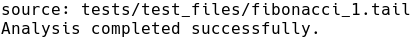
\includegraphics[width=0.7\textwidth]{imagenes/fib1.png}
		\caption{Resultado del análisis de la sucesión de Fibonacci.}
		\label{fig:fib1}
	\end{center}
\end{figure}

Ahora le realizaremos un pequeño cambio al código. En vez de llamar a la función \textit{fib} con el parámetro $3$, lo haremos con \textit{True}. El código se encuentra en \textit{tests/test\_files/fibonacci\_2.tail}.\\

\begin{lstlisting}[style=tail]
fib : Int -> Int
fib(n) :=
	if n <= 1 then
		1
	else
		fib(n-1) + fib(n-2)

write("fib(True) = {fib(True)}")
\end{lstlisting}

El sistema de tipos debería detectar que \textit{True} no es de tipo \textit{Int} y comunicárnoslo, y eso es lo que ocurre. El resultado se puede ver en la figura \ref{fig:fib2}\\

\begin{figure}[H]
	\begin{center}
		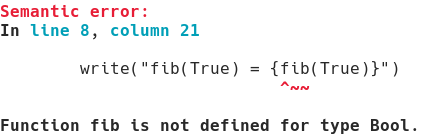
\includegraphics[width=0.7\textwidth]{imagenes/fib2.png}
		\caption{Resultado del análisis de la sucesión de Fibonacci con un parámetro incorrecto.}
		\label{fig:fib2}
	\end{center}
\end{figure}

Cambiaremos de nuevo este código para mostrar como también se detecta cuando una variable no ha sido declarada. Este código se puede encontrar en \textit{tests/test\_files/fibonacci\_3.tail}.\\

\begin{lstlisting}[style=tail]
fib : Int -> Int
fib(n) :=
	if x <= 1 then
		1
	else
		fib(n-1) + fib(n-2)

write("fib(3) = {fib(3)}")
\end{lstlisting}

Se puede ver como se captura el error en la figura \ref{fig:fib3}.\\

\begin{figure}[H]
	\begin{center}
		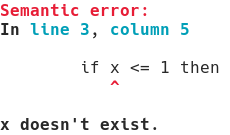
\includegraphics[width=0.35\textwidth]{imagenes/fib3.png}
		\caption{Resultado del análisis de la sucesión de Fibonacci con una variable inexistente.}
		\label{fig:fib3}
	\end{center}
\end{figure}

Modificaremos este código una última vez para ver que ocurre cuando usamos una variable que se nos ha olvidado inicializar. Se puede encontrar este código en \textit{tests/test\_files/fibonacci\_4.tail}.\\

\begin{lstlisting}[style=tail]
fib : Int -> Int
fib(n) :=
	if n <= 1 then
		1
	else
		fib(n-1) + fib(n-2)

x : Int

write("fib(x) = {fib(x)}")
\end{lstlisting}

Como se ve en la figura \ref{fig:fib4} el analizador semántico se da cuenta del fallo.\\

\begin{figure}[H]
	\begin{center}
		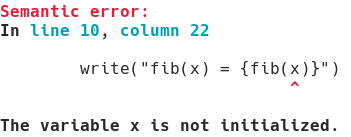
\includegraphics[width=0.55\textwidth]{imagenes/fib4.png}
		\caption{Resultado del análisis de la sucesión de Fibonacci con una variable sin inicializar.}
		\label{fig:fib4}
	\end{center}
\end{figure}

Veamos ahora dos programas que utilizan la unión de tipos. Mientras que el primero es completamente correcto, en el segundo a la variable $x$ se le asigna un valor de un tipo diferente al que se le ha declarado. El código se encuentra en \textit{tests/test\_files/union\_types\_1.tail} y \textit{tests/test\_files/union\_types\_2.tail} respectivamente.\\

\begin{lstlisting}[style=tail]
f : Bool -> :Hola or String

f(b) := if b then :hola else "hola"

x : Atom or String
x := f(True)

write("f(true) = {x}")
\end{lstlisting}

\begin{lstlisting}[style=tail]
f : Bool -> :Hola or String

f(b) := if b then :hola else "hola"

x : Atom or Int
x := f(True)

write("f(true) = {x}")
\end{lstlisting}

El análisis del primer programa termina correctamente, como se muestra en la figura \ref{fig:un1}.

\begin{figure}[H]
	\begin{center}
		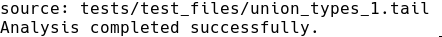
\includegraphics[width=0.7\textwidth]{imagenes/union1.png}
		\caption{Resultado del análisis de la unión de tipos.}
		\label{fig:un1}
	\end{center}
\end{figure}

En el segundo, en cambio, se detecta el error y se muestra por pantalla, siendo visible en la figura \ref{fig:un2}.\\

\begin{figure}[H]
	\begin{center}
		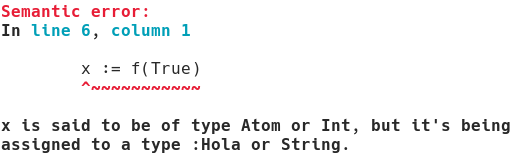
\includegraphics[width=0.75\textwidth]{imagenes/union2.png}
		\caption{Resultado del análisis de una asignación incorrecta con unión de tipos.}
		\label{fig:un2}
	\end{center}
\end{figure}


Hacemos ahora lo análogo con la intersección de tipos. A continuación se muestran dos programas, uno correcto y otro con una asignación del tipo equivocado. El código se encuentra en \textit{tests/test\_files/intersection\_types\_1.tail} y \textit{tests/test\_files/intersection\_types\_2.tail}. En las figuras \ref{fig:in1} y \ref{fig:in2} se muestra la salida de la ejecución.\\

\begin{lstlisting}[style=tail]
x : (:A1 or :A2) and (:A2 or :A3)
x := :a2

write("x = {x}")
\end{lstlisting}

\begin{figure}[H]
	\begin{center}
		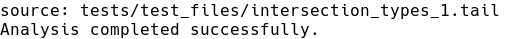
\includegraphics[width=0.75\textwidth]{imagenes/int1.png}
		\caption{Resultado del análisis de la intersección de tipos.}
		\label{fig:in1}
	\end{center}
\end{figure}

\begin{lstlisting}[style=tail]
x : (:A1 or :A2) and (:A2 or :A3)
x := :a3

write("x = {x}")
\end{lstlisting}

\begin{figure}[H]
	\begin{center}
		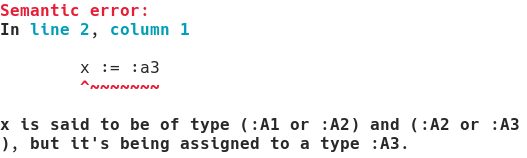
\includegraphics[width=0.75\textwidth]{imagenes/int2.png}
		\caption{Resultado del análisis de la intersección de tipos con una asignación incorrecta.}
		\label{fig:in2}
	\end{center}
\end{figure}


Para terminar comprobamos que el análisis de los tipos graduales funciona correctamente. En este primer fragmento de código, disponible en \textit{tests/test\_files/gradual\_types\_1.tail}, se ve como es posible pasar como argumento valores de diferentes tipos. En la figura \ref{fig:grad1} se muestra que el análisis termina correctamente.\\

\begin{lstlisting}[style=tail]
f : ?, Bool -> ? or String
f(x, b) := if b then x else "Nada"

write("f(3, True) = {f(3, True)}")
write("f(:hola, True) = {f(:hola, True)}")
\end{lstlisting}

\begin{figure}[H]
	\begin{center}
		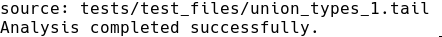
\includegraphics[width=0.7\textwidth]{imagenes/grad1.png}
		\caption{Resultado del análisis de tipos graduales.}
		\label{fig:grad1}
	\end{center}
\end{figure}

En cambio, cuando usamos un argumento del tipo incorrecto en el segundo parámetro, como en el siguiente código, el analizador lo detecta, como se muestra en la figura \ref{fig:grad2}. El código se puede encontrar en \textit{tests/test\_files/gradual\_types\_2.tail}.\\

\begin{lstlisting}[style=tail]
f : ?, Bool -> ? or String
f(x, b) := if b then x else "Nada"

write("f(3, :no_bool) = {f(3, :no_bool)}")
\end{lstlisting}

\begin{figure}[H]
	\begin{center}
		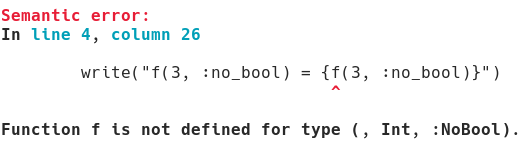
\includegraphics[width=0.8\textwidth]{imagenes/grad2.png}
		\caption{Resultado del análisis de tipos graduales con un argumento incorrecto.}
		\label{fig:grad2}
	\end{center}
\end{figure}

Así, damos por concluida la presentación de diferentes ejecuciones y con ello el capítulo dedicado a la implementación.\\